\chapter{Co-expression of NER repair factors}
The previously described model-aided analysis of the DNA repair process revealed the link between the emergent phenomenon of rapidly exchanging and transiently interacting NER components with the experimentally observed slow first-order kinetics of repair. An important functional consequence of this kinetic design is that the control of the repair rate is shared by all repair factors. This manifests in the mathematical prediction of uniformly distributed response coefficients, which quantify the relative change of the repair rate in answer to changes in the nuclear repair protein concentration. Exploiting the natural variability in NER factor expression, their moderate control on the rate of repair could be experimentally resolved for different repair phases. These findings, however, were made under the assumption of a functional independence of the individual NER components. Effects resulting from co-regulated NER factor expression or protein degradation were so far neglected as a first approximation.  \\
To test this assumption, in the following chapter we will investigate a potential cross-correlation among the involved repair factors experimentally. Surprisingly, we find that the nuclear expression of five pairwise measured repair factors (XPC, TFIIH, XPA, XPF and RPA) is indeed strong positively correlated, whereas there is no correlation with the repair-independent cell cycle marker \textbf{Ki67}. This result suggests an additional control mechanism orchestrating NER factor expression on the transcriptional or translational level.    

- sentence about who did what

\section{Nuclear expression of NER factors is strongly correlated}

\subsection{Microscopy analysis of co-staining experiments}

Using fluorescence microscopy for the quantitative analysis of the NER process proved to result in accurate measurements of the nuclear expression and UV-induced repair dynamics of the individual repair factors at a high signal to noise ratio. This applies for the stably transfected fluorescently tagged repair protein expression as well as for an immunocytochemistry approach with an indirect antibody-labeling of the measured NER factors. The latter technique has the advantage that once a specifically binding antibody is established it can be applied on all cell types containing the desired antigen. On this basis, indirect labeling of the primary antibody with a secondary antibody allows for the combinatorial tagging of multiple antigens restricted only by cross-reactions between antibodies originating from the same host species \cite{Burry2011,Giepmans2006}. Following such a protocol we established five single cell double stainings (cf.\ Table \ref{tab:co-staining} using the primary and secondary antibodies listed in Table \textbf{tbm}. 


\begin{table}[h!]
	\centering
	\begin{tabular}{cccccc}
		\hline
			\rule{0pt}{2ex}
			&\textbf{XPC} & \textbf{TFIIH} & \textbf{XPA} & \textbf{XPF} & \textbf{RPA}\\ \hline
			\rule{0pt}{3ex}
\textbf{XPC}&        X    &           X    & X            &         X    & X            \\ \hline
			\rule{0pt}{3ex}
\textbf{TFIIH}&           & -              & -            & X            & -             \\ \hline
			\rule{0pt}{3ex}
\textbf{XPA}&             &                & -            & X            & X             \\ \hline
			\rule{0pt}{3ex}
\textbf{XPF}&             &                &              & -            & -              \\ \hline
			\rule{0pt}{3ex}
\textbf{RPA}&             &                &              &              & -               \\ \hline
			\rule{0pt}{3ex}
		
	\end{tabular}
	\caption{\textbf{Mean and standard deviation of the variability in nuclear XPC, TFIIH, XPA and XPF expression.} }\label{tab:co-staining}
\end{table}   

Additional two cross-correlation measurements were possible because of a directly labeled monoclonal mouse XPC-antibody. After an initial indirect labeling step for one of the other four repair factors no further secondary antibody is needed. Hence, there is no cross-recognition for primary antibodies from the same species. Moreover, the direct labeling permits a double staining for XPC with two individual fluorophors, which offers a precise estimate of the measurement error (cf.\ Section \ref{natural_Variability_m}). \\
The cross-correlation analysis was performed in	human diploid female fibroblasts which were grown to confluency on coverslips. Analogous to the description in Section \ref{sec:local_irradiation} cells were UV-irradiated locally with a dose of 100 J/$\text{m}^\text{2}$. Pre-incubated with serum-free medium containing 10 \textmu M EdU cells were allowed to repair for 60 minutes in an incubator. After the subsequent direct or indirect antibody labeling of two selected repair factors cells were additionally incubated with a DAPI solution, which visualizes the cell's chromatin and thus the contour of the nucleus. For each double staining microscopic 3-dimensional imaging was conducted on a Leica TCS SP5 II confocal microscope. All images were analyzed following the protocol presented in Section \ref{subsec:AccuFlipExp}. Segmentation of the nucleus was performed on the DAPI signal, due to the large signal-to-nose ratio in this channel (cf.\ Appendix \textbf{Appendix} and Figure \ref{fig:coStaining}A). The segmented region was then used to quantify the signal emitted by the secondary antibodies at 488 and 647 nm (cf.\ Figure \ref{fig:coStaining}B and C). For the same reason segmentation of the locally UV-irradiated chromatin was done with the EdU signal and then projected onto the signal of accumulated protein (cf.\ Figure \ref{fig:coStaining}D).   


\begin{figure}[htbp]
	\begin{center}
		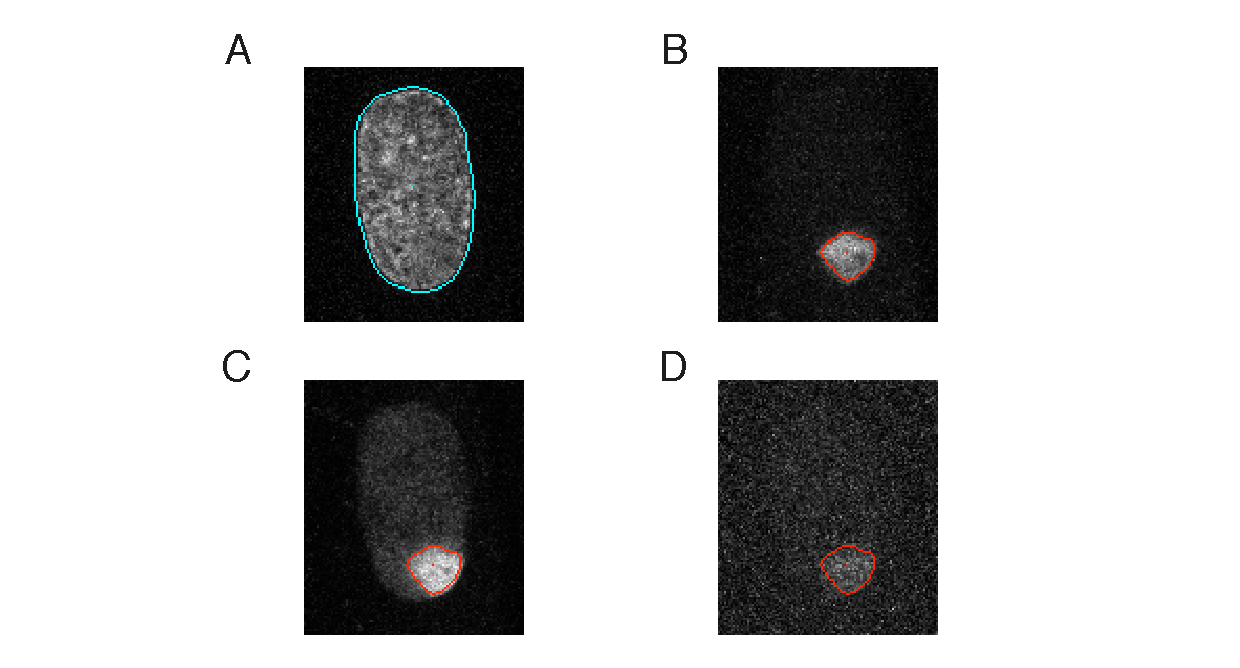
\includegraphics[width=1\textwidth]{Abbildungen/figure4_1.pdf}
		\caption{\textbf{Blubb.} A) B) }
		\label{fig:coStaining}
	\end{center}
\end{figure}


To test whether the antibody co-staining experiment is suitable for the cross-correlation analysis we measured XPC with a directly labeled antibody as well as an indirect labeling. We correlated both signals originating from the entire nucleus including the UV-irradiated region (cf.\ Figure \ref{fig:coExpressionData}). Signal quantification and PCA were performed as described in Section \ref{subsec:AccuFlipExp} and \ref{natural_Variability_m}, respectively. Accordingly, the measurement error was determined with ..., which lies in the same range as the combined approach, with one protein stably expressed and the other indirectly labeled. Hence, also this approach is sufficiently accurate to exploit the natural variability in protein expression for the cross-correlation analysis.\\ 
As it turns out, all pairwise correlations of the measured co-staining experiments (cf.\ Table \ref{tab:co-staining}) are strong positively correlated with correlation coefficients between 0.74 and 0.88 (cf.\ Figure \ref{fig:coExpressionData}B-D and Appendix ...). Notably, the result is indifferent whether the acquired fluorescence signal is taken from the whole cell nucleus including the locally damaged area or only from the undamaged chromatin region (cf.\ Figure \ref{fig:coExpressionData}B-D and \ref{fig:coExpressionData}E-F). This suggests that the correlation of nuclear NER factors is independent of the ongoing repair. As a consequence, we suspect the regulatory mechanism determining the protein concentrations on a preceding level like transcription or translation.  



\begin{figure}[htbp]
	\begin{center}
		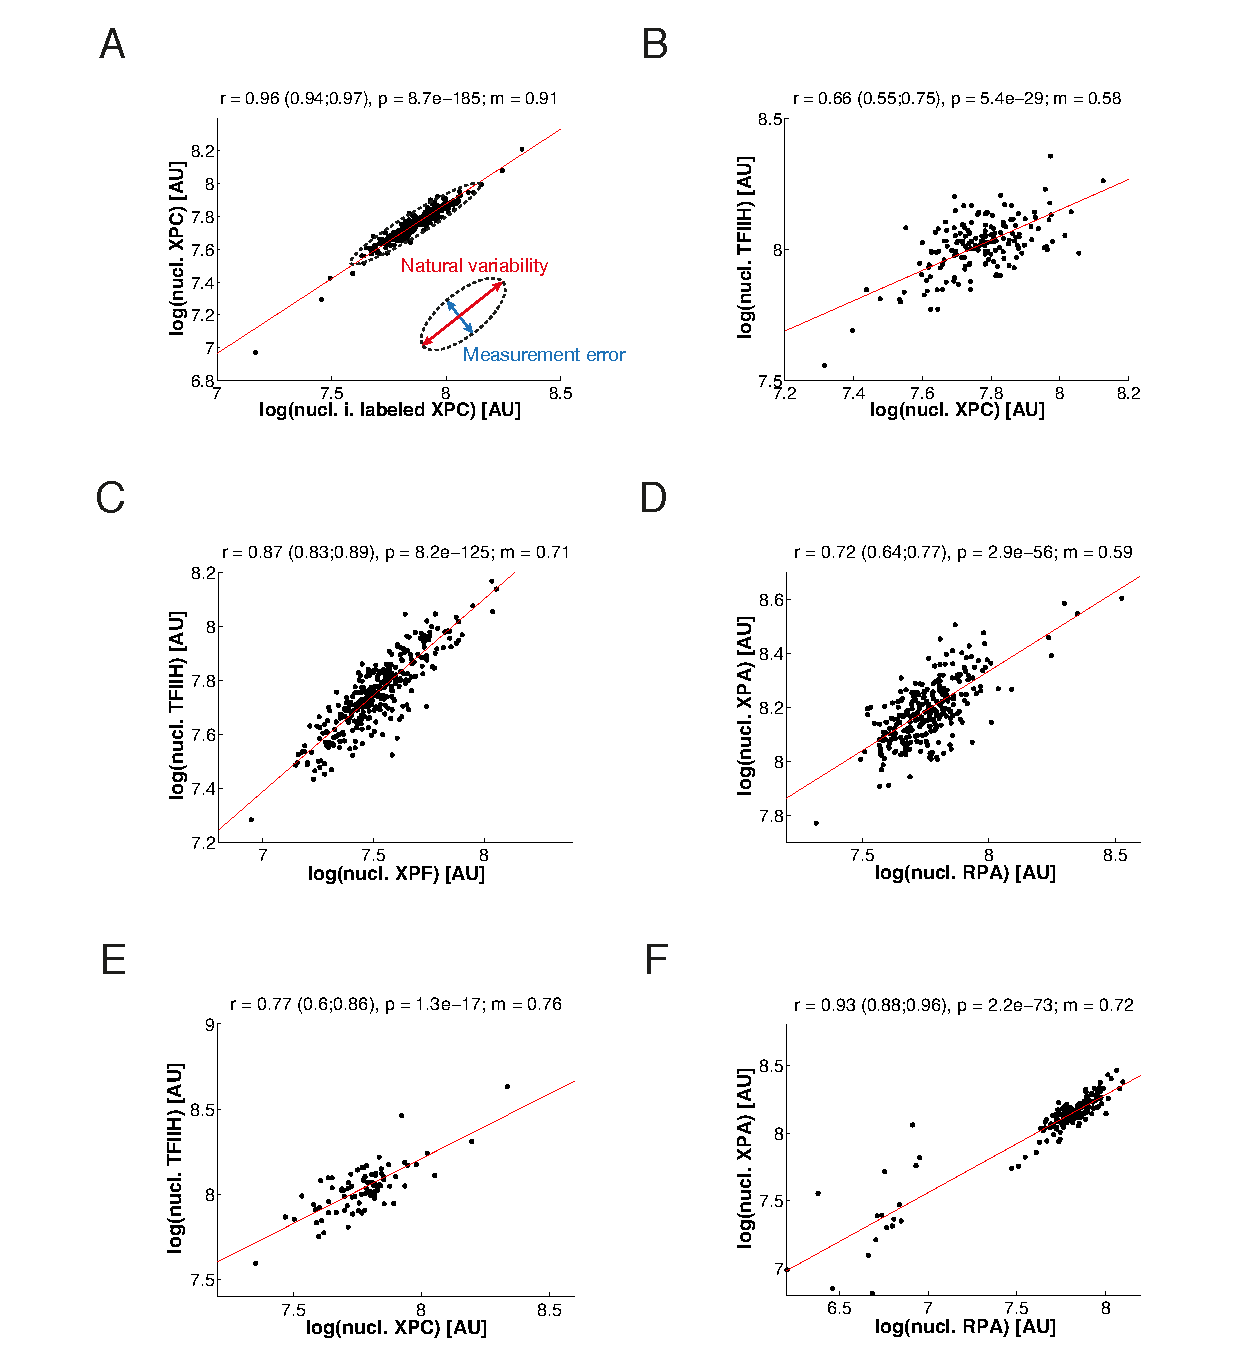
\includegraphics[width=1\textwidth]{Abbildungen/figureTAC_2.pdf}
		\caption{\textbf{NER factor cross-correlation is repair independent.} A) Scatter plot of indirectly antibody-stained XPC against a directly labeled antibody recognizing XPC (n=336) as determined by quantitative (immuno) fluorescence microscopy. B-D) Pairwise correlations of indirectly antibody-labeled XPB against XPC (n=220, B), XPB against XPF (n=410, C) and XPA against RPA (n=350, D) in locally damaged cells. Expression values represent fluorescence intensities originating from the nucleus including the damaged region (signal quantification was performed analogous to \cite{Luijsterburg2010}). E-F) Scatter plots of the nuclear expression of XPB vs. XPC (n=85) and XPA vs. RPA (n=170) in undamaged cells. A-F) Red lines represent linear regression with correlation coefficient r, p-value and slope m. 95\% confidence bounds of all correlation coeffiecients r were estimated by non-parametric bootstrap and are given in brackets. }
		\label{fig:coExpressionData}
	\end{center}
\end{figure}



%\begin{figure}[htbp]
%	\begin{center}
%		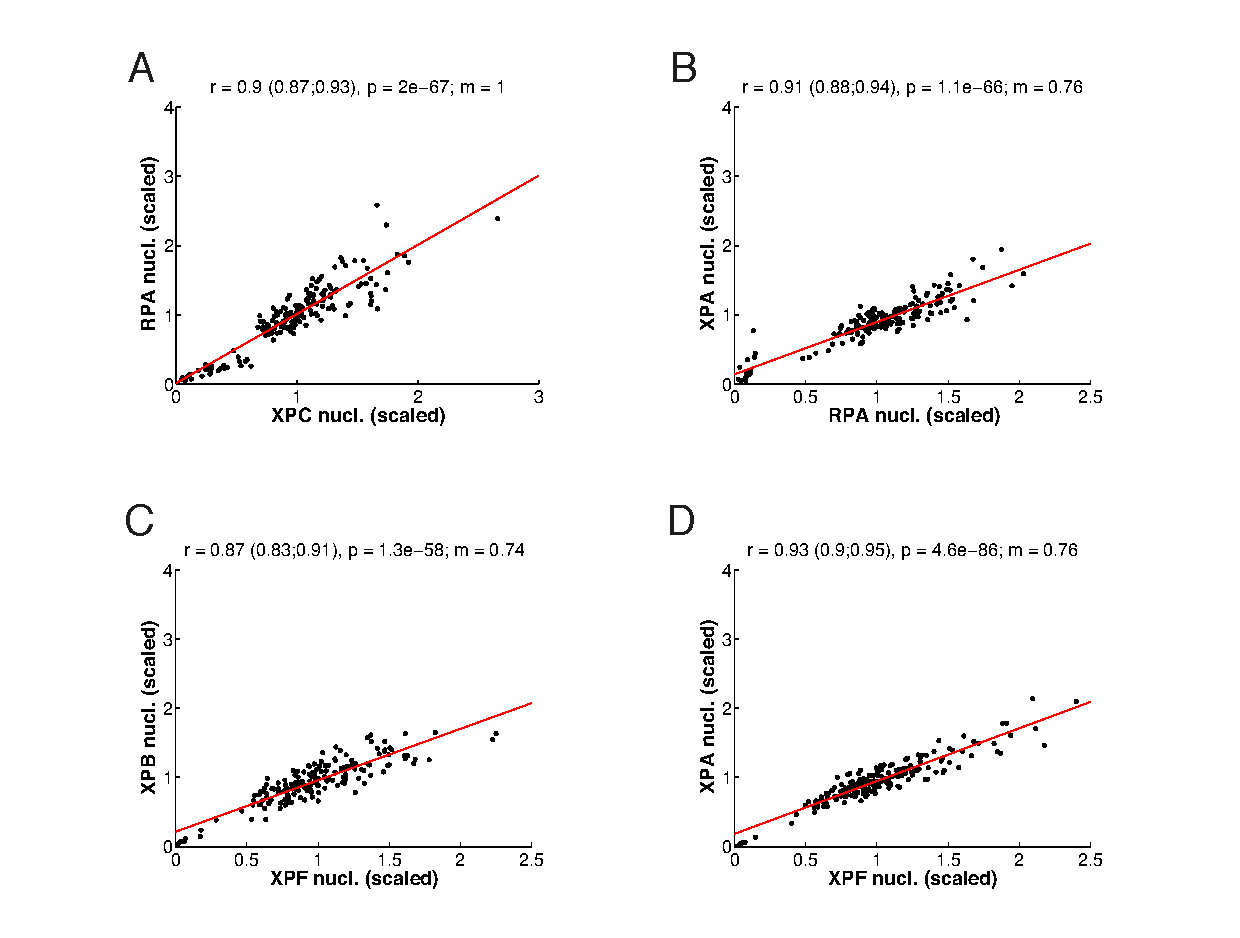
\includegraphics[width=1\textwidth]{Abbildungen/figure4_3.pdf}
%		\caption{\textbf{Blubb.} A) B) }
%		\label{fig:coExpressionData_woDamage}
%	\end{center}
%\end{figure}

\subsection{Flow cytometry}
\begin{figure}[htbp]
	\begin{center}
		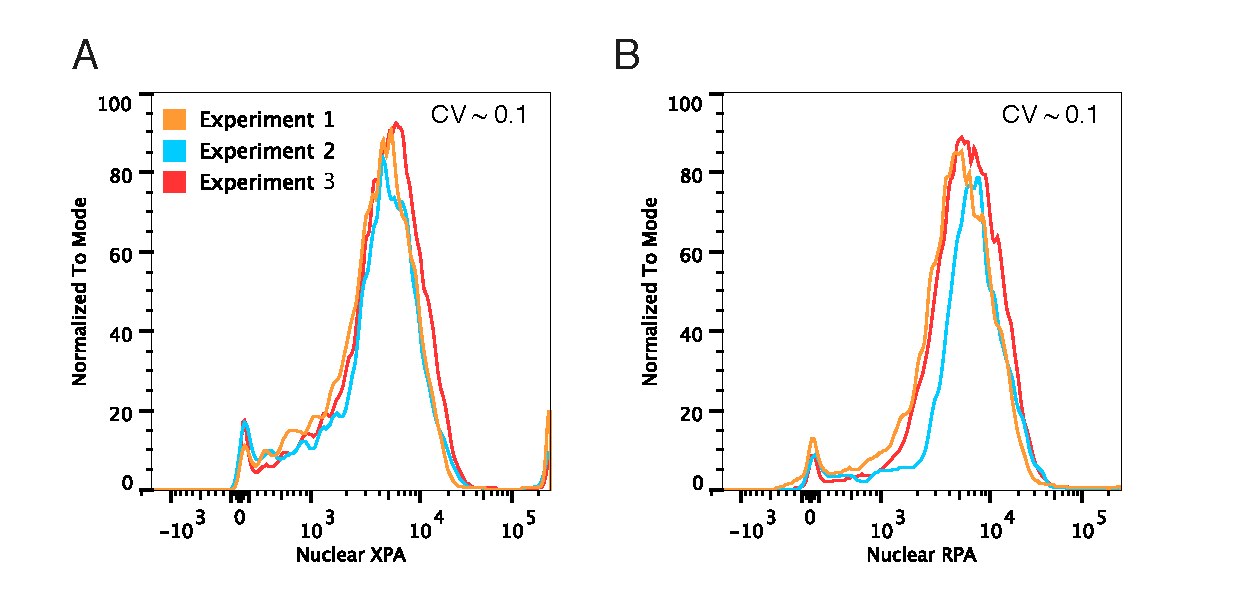
\includegraphics[width=1\textwidth]{Abbildungen/figure4_4.pdf}
		\caption{\textbf{Blubb.} A) B) }
		\label{fig:FC_proteindistribution}
	\end{center}
\end{figure}


\begin{figure}[htbp]
	\begin{center}
		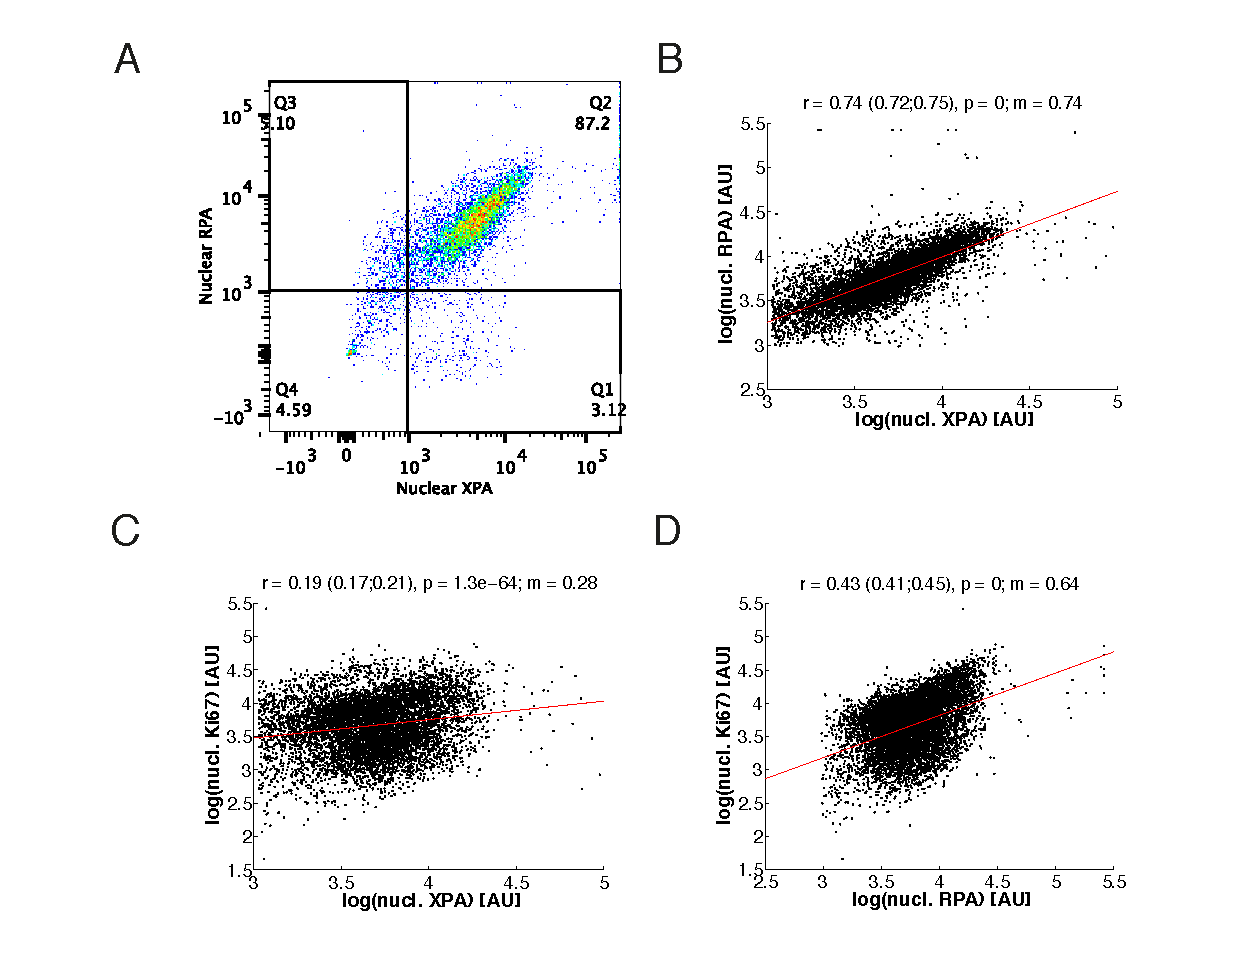
\includegraphics[width=1\textwidth]{Abbildungen/figureTAC_3.pdf}
		\caption{\textbf{Correlated expression of RPA and XPA in human brain pericytes} A) Selection of XPA and RPA positive human brain pericytes (Q2) as determined by flow cytometry (n=8084). B-D) Nuclear expression of indirectly antibody-labeled RPA against XPA (B), Ki67 against XPA (C) and Ki67 against RPA (D). B-D) Red lines represent linear regression with correlation coefficient r, p-value and slope m. 95\% confidence bounds of all correlation coeffiecients r were estimated by non-parametric bootstrap and are given in brackets.}
		\label{fig:FC_correlation}
	\end{center}
\end{figure}

\begin{figure}[htbp]
	\begin{center}
		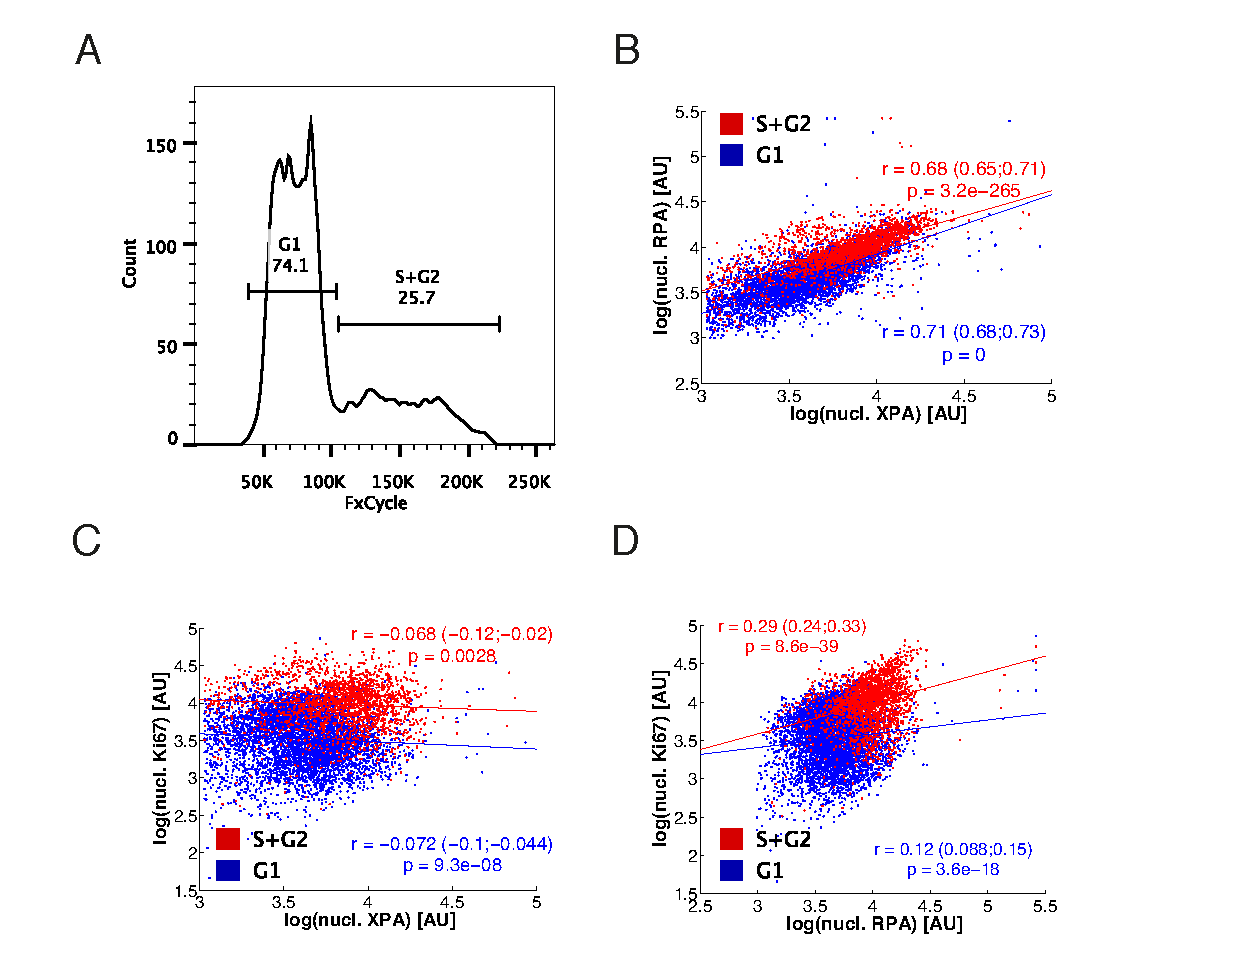
\includegraphics[width=1\textwidth]{Abbildungen/figureTAC_4.pdf}
		\caption{\textbf{NER factor cross-correlation is robust against cell cycle progression.} A) Distribution of fluorescently labeled DNA proportional to the DNA content. Horizontal bars indicate the fractions of cells assigned to G1 (left peak, n=5469) and S+G2 (right peak, n=1945).  B-D) Individual regression analysis of the nuclear expression values sorted according to the corresponding cell-cycle phase (G1 - blue; S+G2 - red) for RPA vs. XPA (B), Ki67 vs. XPA (C) and Ki67 vs. RPA (D). B-D) Red and blue lines represent linear regression with correlation coefficient r and p-value. 95\% confidence bounds of all correlation coeffiecients r were estimated by non-parametric bootstrap and are given in brackets.}
		\label{fig:FC_cell_cycle}
	\end{center}
\end{figure}





\newpage

\subsection{Calibration of the response coefficients}
The positive pairwise correlation of the nuclear repair factor concentration was conclusively shown by two independent experimental approaches. This implies that the abundance of a protein is dependent on the other repair components, which has to be considered when determining the control on the rate of repair. Including this functional interdependence the relation between the measured EdU response (cf.\ Figure \ref{fig:Nuc_vs_DNAsynthesis}) and the response coefficients extends to 

\begin{equation}
 \frac{C_i}{\nu}\frac{d \nu}{d C_i} = \frac{C_i}{\nu}\frac{\partial \nu}{\partial C_i} + \sum_{j \neq i} \left( \frac{C_j}{\nu}\frac{\partial \nu}{\partial C_i}\right) \left(\frac{C_i}{C_j}\frac{\partial C_j}{\partial C_i}\right). 
\end{equation}    

Apart from the unknown response coefficients

\begin{equation}
	R_i = \frac{C_i}{\nu}\frac{\partial \nu}{\partial C_i} \nonumber
\end{equation}

we directly measured the remaining derivatives 

\begin{equation}
A_i = \frac{C_i}{\nu}\frac{d \nu}{d C_i} \nonumber
\end{equation}
as EdU incorporation for varying NER factor concentrations after one hour and

\begin{equation}
B_{ij} = \frac{C_i}{C_j}\frac{\partial C_j}{\partial C_i} \nonumber
\end{equation}

from the regression of repair factor concentration $i$ against repair factor $j$. Hence, for the calculation of the response coefficients we have to solve a linear equation system:

\begin{equation}
	R_i + \sum_{j\neq i} B_{ij}R_j = A_i,
\end{equation}

for $i \in$ 1,...,N. We approximate $B_{ii}$ = 1 and derive the matrix notation $B\vec{R}=\vec{A}$. However, even if we measured all pairwise NER factor dependencies, due to the strong correlations the matrix $B$ would not be invertible.
- Invertierbarkeit...

Although we are not able to derive a specific result for each response coefficient it is possible to make an estimation of their average size. Consider $\nu$ as a function of the concentration of the repair factors $C_i$ and the initial amount of DNA lesions $L$:
\begin{equation}
	\nu = Lf(C_1,...C_N).
\end{equation}
Using, once more, the standard law for the propagation of uncertainty analog to Eqn. ...
 \begin{equation}
 \sigma(\nu) = \sqrt{\sum_{i}\left(\frac{\partial \nu}{\partial C_i}\sigma(C_i) \right)^2 + \left(\frac{\partial \nu}{\partial L}\sigma(L)\right)^2 + \left(\frac{\partial \nu}{\partial C_i} \frac{\partial \nu}{\partial C_i}\textrm{cov}_{ij}\right)^2}
 \end{equation}  
 
 and introducing the response coefficients 
 \begin{equation}
 R_i = \frac{C_i}{\nu}\frac{\partial \nu}{\partial C_i} \nonumber
 \end{equation}
